\chapter{Tribal NeuroSim - Rendszer, Architektúra és Alapok}

\section{Célkitűzés, hatókör és kutatási kapcsolat}
\label{sec:neurosim-24-scope}

A Tribal NeuroSim nem önálló játék, hanem a PremadeGraph gráfelemzési pipeline közvetlen folytatása.
Míg az előző fejezetek a League of Legends meccselőzmények alapján épített játékos-kapcsolati gráfokat elemezték -
klaszterezési módszertan (ld. 10. fejezet) és a két adatkészlet empirikus összehasonlítása (ld. 20. fejezet) révén -,
addig a Tribal NeuroSim ezeket a klaszterprofilokat dinamikus, evolúciós szimulációba viszi tovább.

A kapcsolat szerkezete a következő: a PremadeGraph pipeline minden egyes játékosklasztert
teljesítménymetrikák halmazával jellemez - harci hatékonyság, erőforrás-gazdálkodás, objektívkontroll,
kockázattűrés és csapatkoordináció. Ezek az értékek aggregált klaszterszintű mérőszámokká állnak össze
(\textit{A\_combat}, \textit{A\_resource}, \textit{A\_map\_objective}, \textit{A\_risk}, \textit{A\_team}),
amelyek a Tribal NeuroSim törzseinek iniciális genomszekvenciáját alkotják. Az artifactok
az OpScore és a hozzá kapcsolódó részmetrikák aggregált, klaszterszintre emelt változatai:
a 9.~fejezetben bemutatott teljesítménymetrika adja azt az upstream alapot, amelyből a
szimulációs indulóprofilok létrejönnek.
Az upstream derivációs réteg tehát maga a gráfelemzési eredmény: minden szimulált törzs valódi
meccselőzményből levezetett klaszterprofil alapján indul el, nem mesterségesen megkonstruált paraméterekkel.

A szimulációban egyidejűleg mindkét adatkészlet - a Flex Queue és a SoloQ - klaszterei megjelennek.
Ez a közös versenyterep az alapja a kísérlet komparatív értékének: ha az összes törzs azonos
környezeti szabályok alatt küzd erőforrásokért, területért és túlélésért, akkor megfigyelhető,
hogy a strukturálisan eltérő klaszterprofilok eltérő viselkedési stratégiákat fejlesztenek-e ki.
A kutatási kérdés tehát a következőképpen fogalmazható meg:
\textit{ha Flex Queue-ból és SoloQ-ból derivált klaszterprofilok azonos szimulációs szabályrendszer
alatt versenyeznek, vajon a mögöttes gráfstruktúra mérhető különbséget idéz-e elő az emergáló
túlélési stratégiákban?}

A kísérlet kerete exploratív transzfer-vizsgálat \cite{bonabeau2002}.
Nem kísérel meg közvetlen előrejelzést valódi meccskimenetelekre, és nem állít fel
pszichológiai vagy szociológiai kauzalitást a játékosok viselkedése és a szimulációs eredmények között.
A szimuláció egy modell - explicit feltételezésekkel, meghatározott szabályokkal és reprodukálható
seed-alapú futtatásokkal. Az eredmények tehát nem a valóság közvetlen leképezései, hanem
a választott modell viselkedésének megfigyelései.

Ezen határ explicitálása nem gyengesége a megközelítésnek, hanem annak tudományos erőssége.
Az ágensorientált modellezés irodalmában ez bevett módszertani álláspont: a szimulációs kísérletek értékét
éppen az adja, hogy az összehasonlítás feltételrendszere kontrollált és reprodukálható: azonos
szabályok, azonos kezdeti erőforrás-elosztás, determinisztikus seed-ek.
Az ilyen keretben kapott eredmény - \textit{a flexset klaszterprofilok konvergens stratégiát produkálnak,
a soloq klaszterprofilok változékonyabbat} - a modell viselkedéseként értelmezhető és igazolható,
nem pedig spekulatív általánosításként.

A fejezet hátralévő részei ezt az architektúrát bontják ki: a többügynök-modell és az emergencia
mechanizmusa (22.2), az eseményvezérelt megfigyelhetőség (22.3), a rendszerarchitektúra és
teljesítmény (22.4), valamint a build- és telepítési folyamat (22.5).

\section{Ágensorientált és többügynök-modell}
\label{sec:neurosim-24-abm-mas}

\subsection*{Ágensorientált modellezési keret}

A Tribal NeuroSim ágensorientált modell (ABM): minden törzs önálló döntéshozó egység,
amely kizárólag saját lokális állapota és közvetlen térbeli környezete alapján cselekszik.
Nincs globális optimalizáló, nincs központi irányítás, nincs olyan mechanizmus,
amely a végkimenetelt előre definiálná. A makroszintű minták - terjeszkedés, háborúk,
birodalomkialakulás, kihalás, konszolidáció - kizárólag az egyéni döntések összegzéseként
jelennek meg \cite{bonabeau2002}.

Ez a felépítés szándékos. Az ABM paradigma éppen azt teszi vizsgálhatóvá,
amit a klasszikus analitikus modellek nem: hogyan keletkeznek komplex struktúrák
egyszerű, lokális szabályokból. Egy törzs, amely alacsony élelmiszerkészletére reagálva
szomszédos tile-t igényel, nem „birodalmat épít" - csupán lokálisan racionálisan cselekszik.
A birodalom az ezres nagyságrendű ilyen döntés emergens következménye.

\subsection*{Többügynök-rendszer: decentralizált entitások}

A rendszer többügynök-rendszerként (MAS) is értelmezhető \cite{wooldridgejennings1995}:
minden törzs önálló ágensként működik saját belső állapottal (genomszekvencia, populáció,
élelmiszer, területi kiterjedés, aktív háborúk listája), saját lokális percepcióval
(szomszédos tile-ok biome-ja és tulajdonosa, legközelebbi ellenfél és szövetséges távolsága),
és saját döntési logikával (neurális hálózat, amely a bemeneti jelekből viselkedési hajtóerőket
számít). Az ágensek között nincs közvetlen kommunikáció: interakció kizárólag a közös
térbeli szubsztráton keresztül zajlik - területigénylés, háborúindítás, szövetségajánlat.

Hangsúlyozandó, hogy a törzsek \textit{nem} egyéni játékosokat reprezentálnak.
Minden törzs egy teljes játékosklasztert testesít meg populáció-szintű ágensként:
az iniciális genomszekvenciája az adott klaszter aggregált teljesítményprofilja,
nem pedig egyetlen játékos statisztikája. Ez a skálázási döntés összhangban van
a PremadeGraph upstream rétegének klaszter-alapú elemzési szintjével,
amelyet a 10. fejezet részletez.

\subsection*{Emergáló fázisok a konkrét futtatásokból}

A szimuláció lefolyása minden futtatásban azonos szerkezetű fázisokat mutat,
amelyek nem kódoltak előre, hanem a dinamikából következnek.

Az \textbf{első fázisban} (korai terjeszkedés, kb. tick~0-300) 599 törzs szétszórtan
indítja el területigénylését a hex-rácson. A verseny eleinte implicit: a törzsek
nem egymás ellen harcolnak, hanem a szabad tile-okért versengenek. Az erőforrás-gazdag
biome-ok közelében gyorsabban növekszik a populáció, ami hamarabb éri el a polity-fejlesztési
küszöböket (Tribe → City → Duchy → Kingdom → Empire).

A \textbf{második fázisban} (konszolidáció, kb. tick~300-1000) az erősebb törzsek
fokozatosan felszámolják a gyengébbeket. Háborús deklarációk sűrűsödnek, a túlélők
száma drasztikusan csökken. Az F2 korai futtatás adatai ezt a fázist számszerűsítették:
1452 háborút deklaráltak az 1200 tick során, a csúcsaktivitás ~274 egyidejű aktív
háború volt tick=800 körül. A kihalási ráta ugyanekkor érte el maximumát
(74 törzs/100 tick a tick~900-999 ablakban).

A \textbf{harmadik fázisban} (birodalmi háborúk, kb. tick~1000+) csak a legerősebb
polity-szintű entitások maradnak talpon. A map-ot kevés, de kiterjedt Empire-szintű
törzs uralja; a köztük zajló háborúk döntik el a végkimenetelt. Az első teljes futtatásban
(seed=42, flexset) ez a fázis tick=430-ra 121 élőt, tick=853-ra már csak 36 élőt
hagyott meg, mielőtt egyetlen győztes - Tribe 270, Empire szinten - tick=1707-re
átvette az irányítást 6396 tile felett.

\subsection*{Emergáló dinamikák: háborús kaszkád és szövetség-erózió}

A szimulációban két jellegzetes emergáló dinamika figyelhető meg rendszeresen,
amelyek nem szkriptelt eseményekként, hanem a mechanikák természetes következményeként
jelennek meg.

A \textbf{háborús kaszkád} akkor indul, amikor több törzs egyidejűleg érzékeli ugyanazt
az opportunitást: egy meggyengült domináns szomszéd. Mivel minden törzs önállóan,
lokális információk alapján hoz döntést, a deklarációk szinte szimultán zajlanak.
Ez a dinamika különösen markánsan jelent meg a flexset seed=7777 futtatásban,
ahol tick=2040 körül 55 egyidejű opportunista háború tört ki, és a mező 205-ről
13 élőre zsugorodott 200 ticken belül.

A \textbf{szövetség-erózió} az ellentétes irányból hat: két törzs, amely korábban
szövetségesként viselkedett (kölcsönös meg-nem-támadás), az erőforrás-szűkösség
növekedésével felülvizsgálja ezt az egyensúlyt. Mivel a szövetség bináris
(teljes megnemtámadás vagy teljes háború), az átmenet azonnali és visszafordíthatatlan.
A szövetség-erózió mechanizmusa nem jelent meg minden futtatásban azonos intenzitással,
de megfigyelhető volt mind a flexset, mind a soloq datasetből seeded futtatásokban.
Fontos hozzátenni, hogy a végső, javított futásokban formális szövetségek ritkán
jöttek létre. A mechanika jelen van, de a tényleges makrodinamika többnyire
abszorpcióként jelent meg: a gyengébb törzs ellenállással vagy ellenállás nélkül
beolvadt a nagyobb területi struktúrába.

\subsection*{Az F2 futtatás mint korai ellenőrzési pont}

Az F2 futtatás nem a végleges rendszer bizonyítéka, hanem egy korai, hasznos
ellenőrzési pont. Ebben a verzióban már látható volt, hogy a neurális kimenetek nem
maradnak némák: 599 klaszter-derivált törzs, 1200 tick és flexset adatkészlet mellett
mind a 7 kimeneti hajtóerő aktív volt. Ez akkor fontos mérföldkő volt, mert a korábbi
prototípusokban a szimuláció vagy befagyott, vagy úgy futott le, hogy a döntések
nem okoztak érdemi különbséget a törzsek között.

Az F2-ből ezért csak óvatos következtetés vonható le: ezen a ponton a neurális réteg
már működött, a fitneszértékek elkezdtek szétválni, és megjelent a szelekciós nyomás.
Nem állítható viszont, hogy ez a futás igazolta volna a végleges architektúrát. A későbbi,
2026.~május~16-i és 2026.~május~18-i javítási körök után vált fontossá a determinisztikus,
esemény-alapon visszaellenőrizhető futás, ahol a tile-öröklés, a háború alatti
élelmiszergyűjtés, az artifact-diverzitás és a tombstone-audit már a javított szabályok
szerint működött.

\begin{figure}[h]
\centering
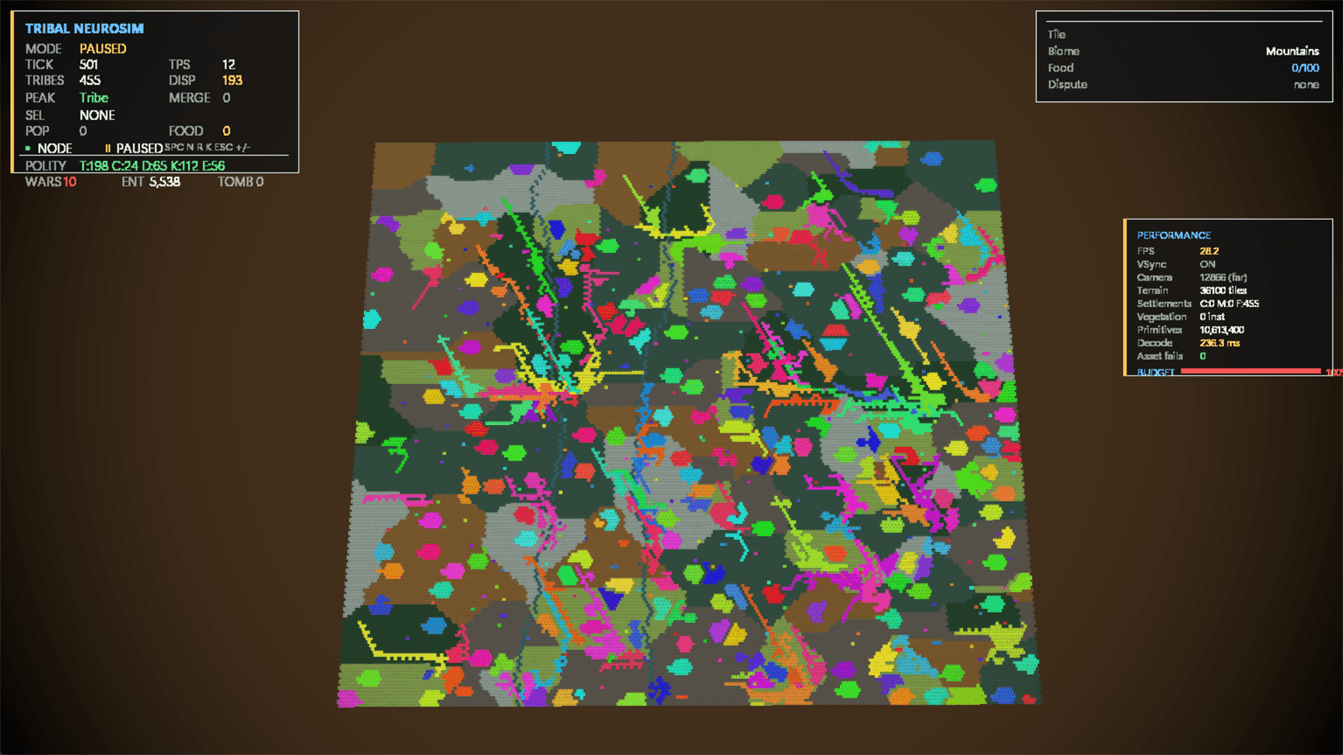
\includegraphics[width=0.9\textwidth]{assets/neurosim/run67fl7777-fl-s7777-tick500.png}
\caption{Flexset seed=7777, tick=500: 455 élő törzs konszolidáció közben.
A területi foltok mérete jelzi az emergáló hatalmi struktúrát.}
\label{fig:neurosim-fl7777-tick500}
\end{figure}

\begin{figure}[h]
\centering
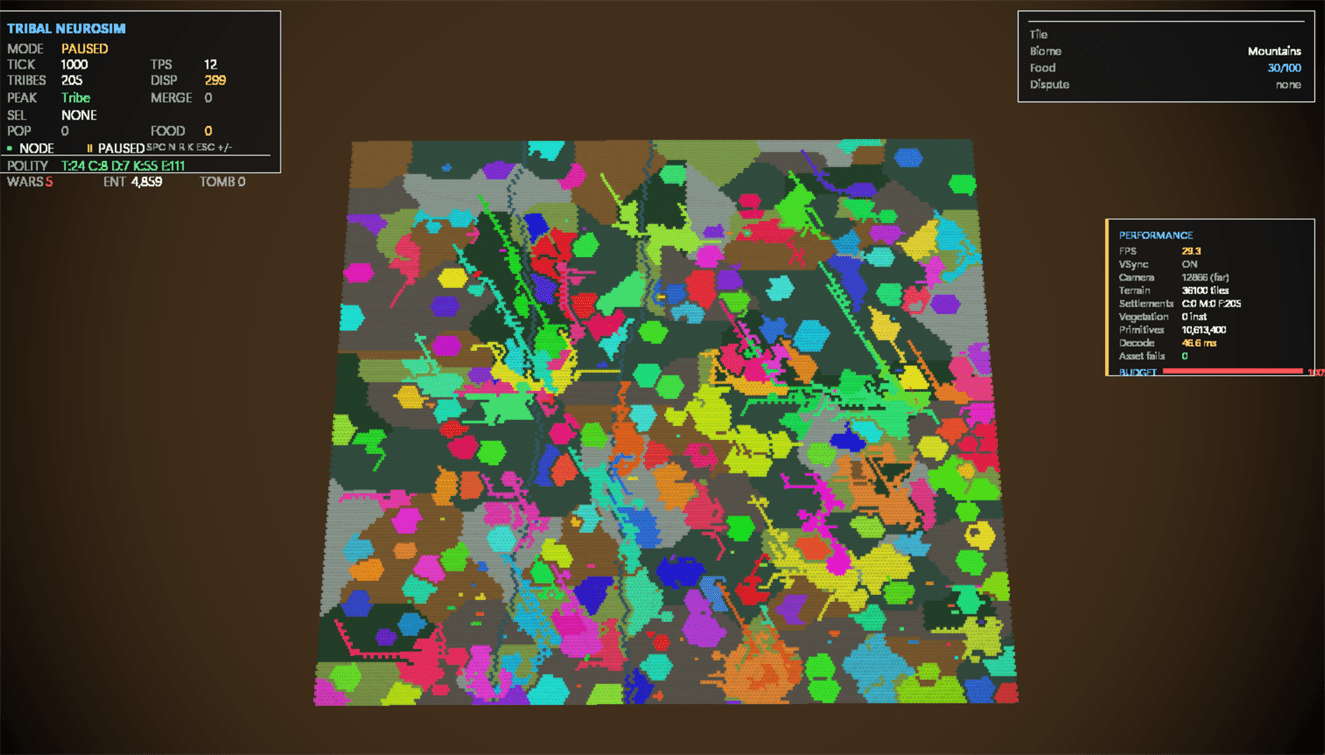
\includegraphics[width=0.9\textwidth]{assets/neurosim/run67fl7777-fl-s7777-tick1000.png}
\caption{Flexset seed=7777, tick=1000: 205 élő törzs, a birodalom-korszak
kezdete. A polity-szint dominanciája látható.}
\label{fig:neurosim-fl7777-tick1000}
\end{figure}

A 20. fejezetben tárgyalt flexset-soloq makroszintű összehasonlítás itt nyer szimulációs
vetületet: az eltérő gráfstruktúrákból derivált klaszterprofilok eltérő emergáló
dinamikákat produkálnak ugyanabban az ABM keretben, ugyanazok alatt a szabályok alatt.

\section{Eseményvezérelt megfigyelhetőség}
\label{sec:neurosim-24-observability}

\subsection*{A végső térképállapot önmagában nem elegendő}

Egy szimuláció tudományos értéke nem merül ki a végső állapot rögzítésében.
Annak megállapítása, hogy melyik törzs nyert, önmagában nem magyarázza a nyerés okát.
Ahhoz, hogy egy törzs túlélése, terjeszkedése vagy összeomlása értelmezhető legyen,
minden lényeges állapotváltásnak nyomkövethetőnek kell lennie: melyik tick-en halt éhen,
melyik háborút nyerte, milyen genommal haladt a következő generációba, és miért hagyott
fel egy szomszédos tile igénylésével.

Ez a felismerés a v2 webes prototípus post-mortem elemzéséből következett közvetlenül.
A korai futtatásban tick=187 körül a populáció közel felére zuhant, de a rendszerben
semmiféle nyom nem maradt arról, miért: nem volt rögzítve a kihalás oka, a törzs azonosítója,
az utolsó élelmiszer-állapot, sem az, hogy háborúban halt-e el vagy éhhalál következtében.
Ugyanebben a futtatásban tick=257-re 323 aktív háborút jelzett a rendszer, miközben
a populáció már jóval alacsonyabb volt ennél - ez volt az első mért jele az úgynevezett
\textit{ghost war} problémának: a halott törzsek háborúi nem szűntek meg,
hanem tovább halmozódtak a memóriában.
A végső állapotban, tick=3085-nél, egyetlen élő törzs állt szemben 182 aktív
szellemháborúval. A szimuláció lefutott, de nem volt interpretálható.

Ez a tapasztalat vezette be a kritikus újratervezés egyik sarokköveként az
eseményvezérelt megfigyelhetőség elvét: a szimulációnak minden lényeges eseményt
strukturáltan kell rögzítenie, az append-only eseménybusz elvét követve \cite{fowler2005}.

\subsection*{Append-only eseménybusz és törzsenként napló}

A v3 architektúrában az eseménynapló két rétegből áll.

A \textbf{globális eseménybusz} append-only gyűrűs pufferként működik: minden kihalás,
háborúdeklaráció, szövetségkötés, generációváltás és intervenciós esemény bekerül
egy időrendezett naplóba. A bejegyzések strukturált rekordok: tartalmazzák az esemény típusát,
a tick és generáció számát, az érintett törzs azonosítóját, és ahol releváns, az ellenfél
vagy az érintett tile azonosítóját is. A bejegyzések a \textit{GET /api/events/recent}
REST endpointon keresztül lekérdezhetők, alapértelmezésként az utolsó 50 bejegyzéssel.

A \textbf{törzsenként napló} minden élő és kihalt törzshöz önálló eseményszálat tart fenn.
A törzs halála nem törli a naplóját: a \textit{GET /api/tribes/\{id\}/events}
endpoint kihalt törzsek esetén is kiszolgál. Ez az utólagos értelmezhetőség
architektúrájának alappillére: a teljes futtatás után visszakereshető, miért halt ki
az adott törzs, milyen háborúkban vett részt, és melyik genomot vitte magával utolsó generációjáig.

\subsection*{Tombstone rekordok: kihalt törzsek auditálható állapota}

A TaskR2 implementáció bevezette a \textit{TombstoneLedger} modult.
Minden törzs halálakor egy \textit{TombstoneRecord} kerül rögzítésre, amely tartalmazza:
a törzs és klaszter azonosítóját, a halál tick-jét és generációját, a populációt és
területet a halál pillanatában, a halál okát (\textit{cause}), a leszármazási összefoglalót,
valamint az öt artifakt-pontszám pillanatfelvételét (\textit{final\_artifacts}).
A rekord mérete ~100 bájt - a kihalt törzs teljes aktív állapotát felváltja
ez a kompakt auditbejegyzés.

A \textit{cleanup\_tribe()} metódus atomikusan hajtja végre a törzs felszámolását:
tombstone rögzítése, majd az összes aktív háború lezárása \textit{WarCancelled}
státusszal, végül a területi igények visszavonása. Ez az atomikus végrehajtás
szünteti meg a ghost war jelenséget: a halott törzs háborúi azonnal eltűnnek
az aktív háborúk listájából.

\begin{figure}[h]
\centering
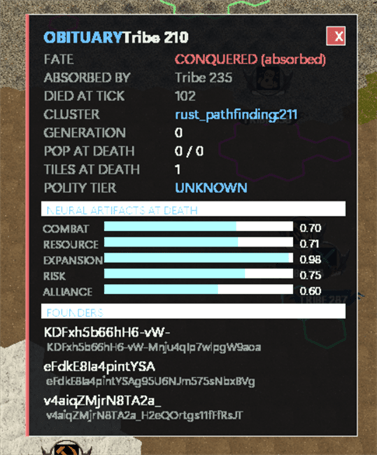
\includegraphics[width=0.82\textwidth]{assets/neurosim/screenshots-orbituary.png}
\caption{Tombstone/obituary nézet: a kihalt törzsek auditálható rekordként maradnak
vissza, nem aktív szimulációs objektumként.}
\label{fig:neurosim-tombstone-obituary}
\end{figure}

\subsection*{Háborús eseménystruktúra}

A TaskL implementáció bevezette a \textit{WarState} adatstruktúrát, amely egy háborút
teljes életciklusán át nyomon követ. Minden háborús rekord rögzíti a háborút indító
és fogadó törzs azonosítóját, az indulás tick-jét, az aktuális státuszt
(\textit{Active}, \textit{Peace}, \textit{AttackerWon}, \textit{DefenderWon}),
a felek veszteségeit harci köröként frissítve, valamint az aktuális csatahelyszín tile-azonosítóját.
A \textit{GET /api/wars/active} endpoint az összes aktív háborút visszaadja
a eltelt tick-szám és kumulált veszteségekkel együtt. A háborúdeklaráció és a kimenetel
(\textit{WarDeclared}, \textit{WarResolved}) mind a globális eseménybuszba, mind az
érintett törzsek saját naplójába bekerül.

\subsection*{JSONL napló a fejnélküli CLI futtatásokhoz}

A headless (\textit{--cli-run}) futtatási módban a szimuláció JSONL formátumú naplót ír
a standard kimenetre. Három típusú bejegyzés váltakozik:
(1)~\textit{checkpoint} rekordok konfigurálható tick-intervallumonként - tartalmazzák
az élő törzsek számát, az aktív háborúkat, a polity-eloszlást és az aggregált
fitnesz-statisztikákat;
(2)~háborús esemény rekordok minden deklarációra és kimenetelre;
(3)~egyetlen \textit{final\_summary} bejegyzés a futtatás végén - rögzíti a győztest,
annak genomprofilját, viselkedési archetípusát, a teljes háborús mérleget, és
az összes kihalt törzs tombstone-összesítőjét.

Ez a napló teszi lehetővé a batch futtatások determinizmus-igazolását: öt párhuzamos
fejnélküli futtatás azonos seed-del azonos \textit{final\_summary} győztes rekordot kell
produkáljon, és ez az egyezés mérhetően ellenőrizhető.

A végjáték értelmezéséhez a térképkép helyett a napló a döntő forrás. A seed=42
flexset futás friss, javított logja például tömören mutatja, hogy a végső szakaszban
nem szövetségi egyensúly, hanem egymást követő abszorpciók és háborús lezárások vezettek
az egyetlen túlélőhöz:

\begin{lstlisting}[language={},caption={Flexset seed=42 végjáték-részlet a javított futás logjából}]
[SIM tick=2400] alive=3 tiles=39368 max_tile=23149 avg_pop=1419769 wars_active=2
[WAR tick=2424] tribe_596 defeated tribe_557 (attacker won)
[SIM tick=2450] alive=2 tiles=39368 max_tile=28161 avg_pop=1314475 wars_active=0
[OPPORTUNITY WAR tick=2460] tribe_90 -> tribe_596 (raid=0.28 aggr=0.84)
[WAR tick=2487] tribe_596 defeated tribe_90 (attacker won)
\end{lstlisting}

\section{Rendszerarchitektúra és teljesítmény}
\label{sec:neurosim-24-architecture}

\subsection*{Hatáskör-megosztás: Rust, C\# MonoGame és Node}

A Tribal NeuroSim v3 háromkomponensű architektúrán alapul, ahol minden réteg
felelősségi köre explicit szerződésben rögzített, és az átfedések szándékosan kerültek.

A \textbf{Rust futtatókörnyezet} az autoritás egyetlen forrása: a tick-ciklust,
a világállapotot, a törzsek neurális döntéshozatalát, a háború- és szövetségfeloldást,
a fuzionálási logikát, a leszármazási regisztert, a tombstone-bejegyzéseket
és az eseménynaplózást mind a Rust bináris kezeli \cite{jung2020}.
Sem a C\# kliens, sem a Node közvetítőréteg nem tart fenn párhuzamos
szimulációs szabályrendszert éles futtatás esetén.
Ez a döntés a 12. fejezetben ismertetett Rust-futtatókörnyezeti elvek közvetlen
kiterjesztése a szimulációs tartományra.

A \textbf{C\# MonoGame kliens} kizárólag vizualizáció és operátori felület:
kamera, térkép-renderelés, törzsinspekciós panel, HUD, artifact-sávok, háborús jelzők.
A kliens nem igazságforrás - a Rust által szolgáltatott keretadatot jeleníti meg,
és lokális demó-harnesszel rendelkezik vizuális teszteléshez (\textit{--empire-stress},
\textit{--dispute-stress}), de ez nem a valódi termék futtatási útja.

A \textbf{Node réteg} vékony közvetítő: összekötőhíd a MonoGame és a Rust szerver
között, dataset-export, indítási konfiguráció és batch-orchestráció kezelője.
Szimulációs logikát nem tartalmaz; minden parancsot és keretfolyamot változtatás nélkül
proxyzik a Rust felé.

\begin{figure}[h]
\centering
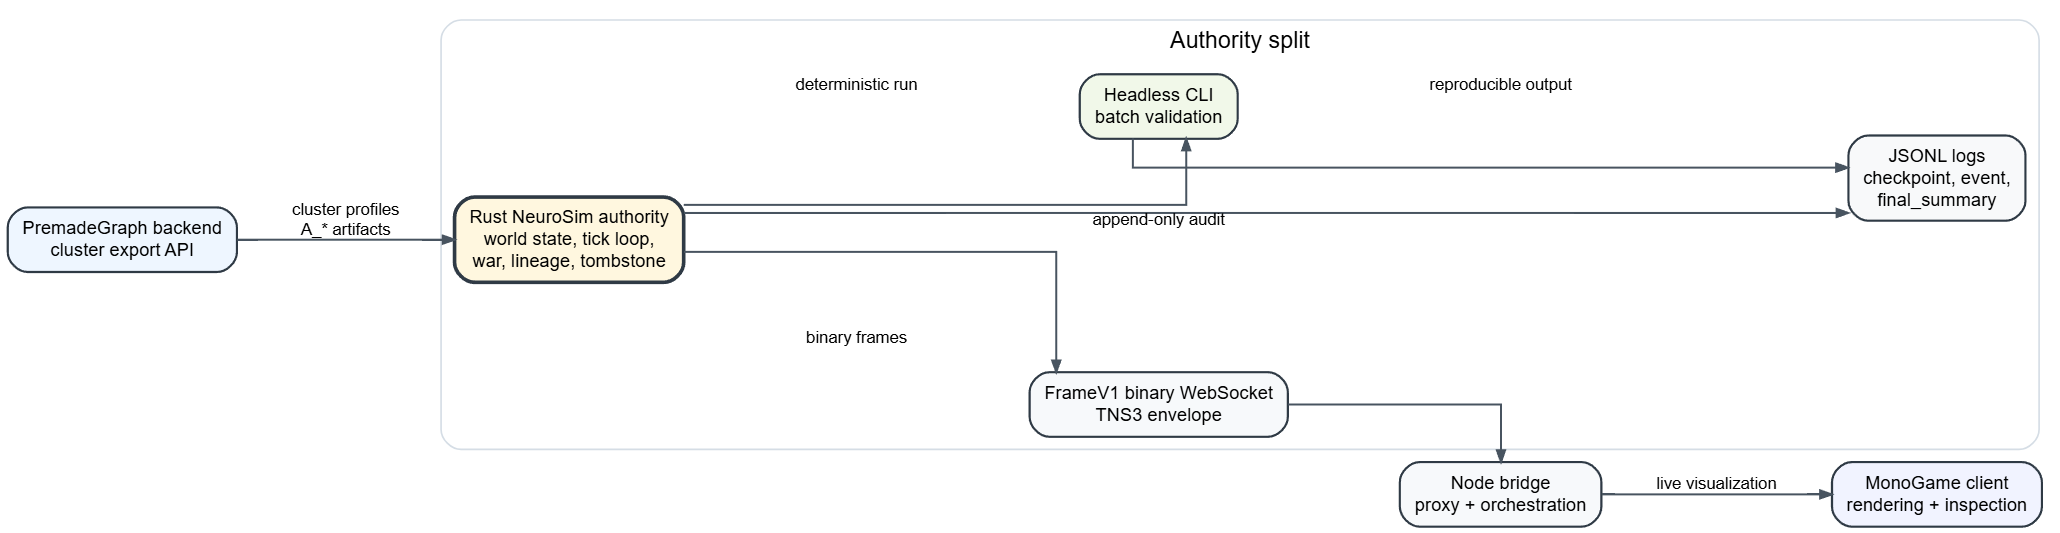
\includegraphics[width=0.92\textwidth]{assets/diagrams/thesis_neurosim_architecture_graphviz.png}
\caption{A Tribal NeuroSim hatáskör-megosztása: a Rust motor az autoritatív szimulációs állapot forrása, míg a Node és MonoGame rétegek közvetítő és megjelenítő szerepet kapnak.}
\label{fig:neurosim-architecture-graphviz}
\end{figure}

E felosztást a böngészőalapú v2 prototípus közvetlen tanulsága motiválta:
ahol a szimulációs állapot az UI-réteghez volt csatolva, ghost war jelenség,
memóriaszivárgás és nem-determinisztikus viselkedés keletkezett.
Az authority split strukturálisan kizárja e hibaosztályokat, mert a végeredmény
egyetlen Rust folyamat belső állapotától függ, nem UI-oldali értelmezéstől.

\subsection*{FrameV1 bináris protokoll}

A Rust szerver és a MonoGame kliens bináris WebSocket kereteken kommunikál.
A protokollt a TaskR7 Rust-oldali implementációja definiálta, a TaskM1 C\# dekóder
implementálta.

Minden keret egy 40 bájtos \textit{TNS3} envelope-pal kezdődik (little-endian):

\begin{table}[h]
\centering
\caption{FrameV1 desktop envelope fejléc.}
\label{tab:framev1-envelope}
\begin{tabular}{rll}
\hline
\textbf{Offset} & \textbf{Méret} & \textbf{Mező} \\
\hline
0  & 4 B & Magic: \textit{"TNS3"} \\
4  & 2 B & Version: \textit{1} \\
6  & 2 B & HeaderBytes: \textit{40} \\
8  & 2 B & PayloadKind: \textit{2} (\textit{FrameV1}) \\
10 & 2 B & Flags \\
12 & 4 B & PayloadBytes \\
16 & 8 B & Tick (\textit{u64}) \\
24 & 4 B & Generation (\textit{u32}) \\
28 & 4 B & RecordCount (élő törzsek száma) \\
32+ & változó & V1 payload \\
\hline
\end{tabular}
\end{table}

A payload section-alapú és önleíró: per-törzs rekordok (50 bájt/törzs)
után opcionálisan tile-rekordok (\textit{FLAG\_TILE\_DATA = 0x01}, 9 bájt/tile),
háborús rekordok (\textit{FLAG\_WAR\_DATA = 0x02}, 21 bájt/háború),
és esemény-deltók (\textit{FLAG\_EVENT\_DATA = 0x04}) következnek.
A tile-rekordok csak elfoglalt vagy vitatott tile-okra szűkülnek,
így a hasznos terhelés arányos az aktuális aktivitással, nem a teljes térképmérettel.

A bináris formátum döntése teljesítményi és architekturális: JSON sorosítás esetén
a szimulációs tick-ciklus átbocsátóképessége összekapcsolódna a UI renderelési
ciklusával. Little-endian bináris frameknél a Rust szerver 40~ms alatt
lekezel 599 törzs állapotát, miközben a MonoGame kliens aszinkron dekódol és renderel.

Miért hatékony ez a megközelítés? Három okból. Először: a JSON sorosítás elkerülése.
Egy 599-törzsös világ JSON-alapú frissítése tick-enként ~150--200~kB felesleges szöveges
overhead-et generálna; a bináris FrameV1 ugyanezt 50~bájt/törzs + 9~bájt/aktív tile
formátumban kezeli. Másodszor: szekció-szelektivitás. A tile-rekordok csak elfoglalt
vagy vitatott tile-okra szűkülnek (\textit{FLAG\_TILE\_DATA = 0x01}), így a payload
arányos az aktivitással, nem a teljes térképmérettel. Harmadszor: szimulációs és
UI-ciklus szétválasztása. A Rust szerver 40~ms alatt lekezel egy teljes 599-törzsös
tick-et; a MonoGame kliens aszinkron dekódol és renderel, anélkül hogy blokkolná a
szimulációs ciklust. A két folyamat egymástól függetlenül fut, ez az architektúra
alapja annak, hogy a szimuláció egyenletesen fut magas törzsszámnál is.

\subsection*{Teljesítményproblémák és megoldásuk}

A 599-klaszteres világ bevezetésekor négy teljesítményszűkületet azonosítottunk.

A legsúlyosabb hotspot az összes-pár szomszédossági keresés volt.
A korai kód minden törzsnél az összes többi törzs összes tile-ját pásztázta végig:

\begin{lstlisting}[language={},basicstyle=\ttfamily\scriptsize,breaklines=true,caption={Régi all-pairs tile-scan: O(n\textsuperscript{2} × tiles) bottleneck}]
let my_tiles = self.tribes[i].territory.iter().copied().collect::<HashSet<_>>();
for other in &self.tribes {
    for tile in &other.territory {
        if self.world.adjacent_tiles(*tile as usize)
            .iter()
            .any(|a| my_tiles.contains(&(*a as u16))) {
            // neighboring tribe found
        }
    }
}
\end{lstlisting}

599 törzsnél ez O($n^2 \times \text{tiles}$) keresést jelentett minden 20-tickes kötegben.
A megoldás két gyorsítótár bevezetése volt:
\textit{tile\_tribe\_idx} (\textit{Vec<u32>}: tile~→~tulajdonos törzs indexe, O(1) lookup)
és \textit{tribe\_id\_to\_idx} (\textit{HashMap<u32, usize>}: törzs id~→~tömb-index, O(1)).
A gyorsítótár tick elején újraépül: ~36\,100 + 599 ≈ 36\,700 egyszerű értékadás,
amelyek után a szomszéddetektálás O($\text{my\_tiles} \times 4$) keresi a szomszédos
tulajdonost.

A vitás tile-ok nyilvántartójában O($n$) lineáris keresést szintén az O(1)
\textit{tribe\_id\_to\_idx} cache váltotta ki.
A hot-path naplózást - 599 törzsnél tickenként százas nagyságrendű \textit{println!}
hívás - a \textit{headless} flag gátolja le; I/O csak checkpoint- és eseménybejegyzéseknél
keletkezik.

\subsection*{Determinizmus-hiba és javítása}

A megfigyelhetőségi igény mellé szimmetrikus követelményként társul a reprodukálhatóság:
azonos seedből azonos kimenetnek kell következnie. Ez v3 fejlesztés során
egy látens hiba miatt nem teljesült.

\textbf{A hiba:} azonos seed egymást követő MonoGame futtatások között különböző
győztest produkált.

\textbf{Gyökérok:} a \textit{set\_clusters()} metódus rendezés nélkül fogadta
a klaszterlistát. A mögöttes SQLite-lekérdezés \textit{ORDER BY} záradék hiányában
tetszőleges sorrendben adta vissza a sorokat, így a törzsek hex-rácsra való
elhelyezési sorrendje futtatásról futtatásra változott.
A szimuláció tick=0-ban divergált - egyetlen neurális döntés megszületése előtt.

\textbf{Javítás:} egyetlen sor a \textit{set\_clusters()} metódusban,
a szimuláció inicializálása előtt:

\begin{lstlisting}[language={},caption={Determinizmus-javítás: klaszterek rendezése azonosító szerint}]
clusters.sort_by(|a, b| a.id.cmp(&b.id));
\end{lstlisting}

\textbf{Igazolás:} CLI mód (fejnélküli, seed=7777) és Docker-en futó MonoGame kliens
(seed=7777) tick=100-nál azonos kimenetet produkált:

\begin{lstlisting}[language={},caption={Determinizmus-ellenőrzés: CLI és MonoGame egyező eredménye tick=100-nál}]
alive=593 | City:41 | Tribe:552
\end{lstlisting}

A reprodukálhatóság a kísérleti eredmények tudományos értékének alapfeltétele:
csak olyan megfigyelés értelmezhető a modell viselkedéseként, amely azonos
körülmények között megismételhető.

\subsection*{Fejnélküli CLI mód}

A rendszer \textit{--cli-run} flag-gel fejnélküli módban futtatható:
nincs HTTP szerver, nincs WebSocket stream, a szimuláció szinkron fut
a végkimenetelig. Ez a mód a batch-validáció és az automatizált reprodukálhatóság-ellenőrzés
elsődleges eszköze.

Kimenet: \textit{logs/neurosim-\{seed\}-\{dataset\}-\{nonce\}.jsonl}.
Három bejegyzéstípus váltakozik: checkpoint rekordok konfigurált tick-intervallumonként,
háborús eseménybejegyzések minden deklarációra és kimenetelre,
és egyetlen \textit{final\_summary} sor a futtatás végén.
A \textit{final\_summary} tartalmazza a győztes azonosítóját, genomprofilját,
viselkedési archetípusát, a teljes háborús mérleget és a tombstone-összesítőt.

Öt párhuzamos fejnélküli futtatás azonos seeddel azonos \textit{final\_summary}
győztes rekordot kell produkáljon. Ez az egyezés mérhető és automatikusan ellenőrizhető,
és erősebb bizonyíték, mint egy önmagában álló végjáték-screenshot.

A CLI futtatások teljes argumentumkészlete:
\begin{lstlisting}[language={},caption={CLI argumentumok és hatásuk}]
--cli-run            Fejnelkuli mod: nincs HTTP/WebSocket, szinkron futtas vegkimenetelig
--seed <u64>         Determinisztikus seed (pl. 42 vagy 7777)
--use-dataset-export Klaszterprofil betoltese a PremadeGraph backendbol
--require-dataset-export  Megszakitja a futtatast ha a backend nem elerheto
--ticks <u64>        Maximalis tick szam (alapertelmezs: 100000)
--checkpoint-interval <u32>  Checkpoint rekord irasanak gyakorisaga (tick)
--clusters <u32>     Szintetikus klaszterek szama (--use-dataset-export nelkul)
\end{lstlisting}

A \textit{--require-dataset-export} flag biztosítja, hogy a batch validáció
soha ne fusson szintetikus adattal ha az a szándék valódi klaszterprofilok használata.
A \textit{--checkpoint-interval 500} érték 599 törzsnél körülbelül 5--7 bejegyzést
ír minden checkpoint-alkalomnál, ami az I/O overhead és az elemezhetőség optimális
kompromisszuma volt a hosszú futtatásoknál.

\section{Build folyamat és telepítés}
\label{sec:neurosim-24-build}

A Tribal NeuroSim futtatási útvonala három rétegre bontható: adatexport,
Rust szimuláció és opcionális vizualizáció. A thesis szempontjából az első kettő
a lényeges, mert ezek adják a reprodukálható JSONL naplókat.

\begin{table}[h]
\centering
\caption{NeuroSim futtatási munkafolyamat.}
\label{tab:neurosim-build-flow}
\begin{tabular}{lll}
\hline
\textbf{Lépés} & \textbf{Feladat} & \textbf{Kimenet} \\
\hline
1 & PremadeGraph backend indítása & klaszterexport API \\
2 & Rust backend release fordítása & \textit{neurosim-backend.exe} \\
3 & Fejnélküli CLI futtatás & JSONL eseménynapló \\
4 & Batch ellenőrzés & ismételhető \textit{final\_summary} \\
5 & MonoGame kliens & élő FrameV1 vizualizáció \\
6 & Docker stack & konténeres demonstráció \\
\hline
\end{tabular}
\end{table}

A klaszterprofilokat a PremadeGraph backend szolgáltatja a
\textit{/api/neurosim/clusters} endpointon keresztül. A Rust bináris a
\textit{PREMADEGRAPH\_URL} és \textit{PREMADEGRAPH\_DATASET\_ID} környezeti
változókból olvassa ki, hogy flexset vagy soloq adatkészletből inicializáljon.

\begin{lstlisting}[language={},basicstyle=\ttfamily\scriptsize,breaklines=true,caption={Egy helyre gyűjtött fejlesztői futtatási parancsok}]
# PremadeGraph backend
npm run dev

# Rust release build
cd backend/genetic-neurosim/backend
cargo build --release

# Reprodukálható CLI futás
$env:PREMADEGRAPH_URL = "http://localhost:3001"
$env:PREMADEGRAPH_DATASET_ID = "flexset"
.\target\release\neurosim-backend.exe --cli-run --seed 7777 --use-dataset-export --checkpoint-interval 500

# Batch determinizmus-ellenőrzés
.\run-batch.ps1 -Runs 5 -Seed 42 -DatasetId flexset
\end{lstlisting}

Élő vizualizáció esetén a Rust szerver FrameV1 WebSocket streamet szolgáltat,
a C\# MonoGame kliens pedig ehhez csatlakozik. Ez a mód demonstrációra alkalmas,
de a tudományos ellenőrzés alapja továbbra is a fejnélküli JSONL napló, mert abban
minden checkpoint, háborús esemény, tombstone rekord és végső összegzés
géppel visszaolvasható.

A Docker Compose konfiguráció ugyanazt a szerződést tartja meg konténeres környezetben:
a \textit{neurosim} service csak akkor indul, ha a PremadeGraph backend healthcheck-je
sikeres, és a klaszterexport endpoint elérhető.
A seed a \textit{NEUROSIM\_WORLD\_SEED} változóval vezérelhető;
az adatkészlet a \textit{PREMADEGRAPH\_URL} által mutatott backend aktív datasetje lesz,
hacsak a \textit{PREMADEGRAPH\_DATASET\_ID} expliciten meg nem adott.

\bigskip
